\section{Antiparticle-to-Particle Ratios}\label{section:star_ratios}
The following steps were taken to correct an  identified antiparticle to particle (pion, kaon, proton and their antiparticle) multiplicity ratios as a function of $p_\textrm{T}$ in three ranges of $\xi$:
\begin{itemize}
	\item The raw identified particle yields were obtained through multi-Gaussian fits to the $n\sigma^i_{dE/dx}$ distributions (Sec.~\ref{section:star_PIDdEdx}), where the vertex reconstruction and energy loss corrections~\cite{supplementaryNote} were applied. The latter depends on the particle type.
	\item The non-SD background was subtracted.
	The~accidental background contribution is very small, hence, any particle-antiparticle differences have a~negligible effect on the result. Therefore, 
	 it was assumed that the~accidental background does not depend on the particle type and for this reason it was not subtracted. 
	\item The particle yields were corrected for track reconstruction efficiencies~\cite{supplementaryNote}, which depend on the particle type and charge. These corrections were averaged over $\eta$ and $V_{z}$.
	The~ratio of particle to antiparticle TPC-TOF efficiencies is shown in Fig.~\ref{fig:ratios_efficiency}.  It weakly depends on $\xi$ range, therefore, only sample results for single range of $0.02<\xi<0.05$  are presented.
	\item The background from non-primary tracks was subtracted (Sec.~\ref{section:star_background_primary}):
	\begin{itemize}
		\item $\pi^\pm$: weak decays pions, muon contribution and background from  detector dead-material interactions,
		\item $p$: background from  detector dead-material interactions,
		\item $p,\bar{p}$: reconstructed tracks which have the appropriate number of common hit points with true-level particle, but the distance between them is too large (this background is negligibly small for other particle types),
		\item fake track contribution was assumed to be the same for each particle type, hence, it was not subtracted. 
	\end{itemize}
	\item Since  track and $\xi$ migrations, and BBC-small efficiency, do not depend on the particle type and charge, these corrections are not applied.
	%Then the tracks were corrected for track and $\xi$ migrations, and BBC-small efficiency, which do not depend on the particle type and charge.
	\item Finally, each antiparticle $p_\textrm{T}$ distribution was divided by the corresponding particle $p_\textrm{T}$ distribution to obtain fully corrected identified antiparticle to particle multiplicity ratios.
	\item Additionally, the average antiparticle to particle ratios over fiducial
	region of $p_\textrm{T}$ in each $\xi$ region were calculated.
	
	%Additionally, the average antiparticle to particle ratios in each $\xi$ region were calculated by fitting a~constant to above ratios.
\end{itemize}

\begin{figure}[h!]
	\centering
	%\vspace{-2.5cm}
	\begin{subfigure}{.49\textwidth}
		\includegraphics[width=\textwidth,page=7]{chapters/chrgSTAR/img/ratiosEffi/correction.pdf}
	\end{subfigure}
	\begin{minipage}{.49\textwidth}
		\caption{Ratio of particle to antiparticle TPC-TOF efficiencies for $0.02<\xi<0.05$.}
		\label{fig:ratios_efficiency}
	\end{minipage}
	
	%\vspace{-1.5cm}
	%\vspace{-2cm}
\end{figure}